\documentclass[11pt,a4paper]{article}
\usepackage[T1]{fontenc}
\usepackage{lmodern}
\usepackage[margin=2.5cm]{geometry}
\usepackage{booktabs}
\usepackage{graphicx}
\usepackage[hidelinks]{hyperref}
\usepackage{microtype}
\usepackage{float}
\setlength{\parskip}{0.5em}
\setlength{\parindent}{0pt}

\title{Two small piano models: notes and measurements}
\author{Hermes Reisner}
\date{November 2026}

\begin{document}
\maketitle

These notes collect what was built, how it was trained and what was measured for the two models in this
repository. They are a record of one project, not a study: the test sets are small, there is one training run per
setting, and nothing was rated by listeners. Every number comes from the scripts in the repository or from the
training logs.

\section{The two models}

\textbf{v1} is a GPT-2 decoder (12 layers, width 768, 12 heads, 87.0M parameters) trained from scratch on
MAESTRO v3 \cite{maestro}. It continues a piano passage given as MIDI. \textbf{v2} is an RWKV-7 \cite{rwkv7}
(12 layers, width 768, head size 64, 93.4M parameters) trained on Aria-MIDI \cite{ariamidi}. It was built for
background music in a game: it has to play for as long as the game runs, follow a density and a loudness setting
every five seconds, and cost little enough per token to run on a laptop next to the game.

\section{Data and tokens}

\textbf{v1.} The 1,276 MAESTRO files are split at random by file (seed 42) into 1,148 training, 63 validation
and 65 test files. This is not MAESTRO's official split, so related performances can land on both sides, which
flatters the validation loss. Each training file is also transposed by $-3$ to $+3$ semitones when every note
stays within the piano's range, which gives 7,569 training sequences. Tokens are MidiTok's REMI
\cite{remi,miditok} with 32 velocity levels, sustain pedal, tempo and time signature, 423 tokens in all.

\textbf{v2.} The pruned, de-duplicated Aria-MIDI release has 820,944 files, 4.59 billion tokens and 1.52 billion
notes in Aria's tokenization (\texttt{ariautils}). 1\,\% of the recordings are held out for validation, chosen by
a hash of the recording id. Files shorter than 1,025 tokens are skipped, which leaves 757,367 training and 7,621
validation files. The 2,144 Aria tokens that occur in the data are kept; 15 control tokens are added.

Aria tokens are timed absolutely: every note has an onset in milliseconds within the current five seconds, and a
\texttt{<T>} token starts each new five seconds. After every \texttt{<T>}, v2 sees two control tokens for the
coming five seconds (Table~\ref{tab:levels}). In training they are computed from the real notes; they are inputs
only and never predicted. 15\,\% of the segments get a ``none'' token for both, so the model also learns to play
without controls, which classifier-free guidance needs.

\begin{table}[h]
\centering\small
\begin{tabular}{lll}
\toprule
Control & Measured over the next 5 s & Levels \\
\midrule
Density & notes per second & 8: below 0.5, 1.5, 3, 5, 8, 12, 18, and above \\
Loudness & mean velocity of the notes & 5: below 45, 55, 65, 75, and above \\
\bottomrule
\end{tabular}
\caption{Control levels.}
\label{tab:levels}
\end{table}

\begin{figure}[h]
\centering
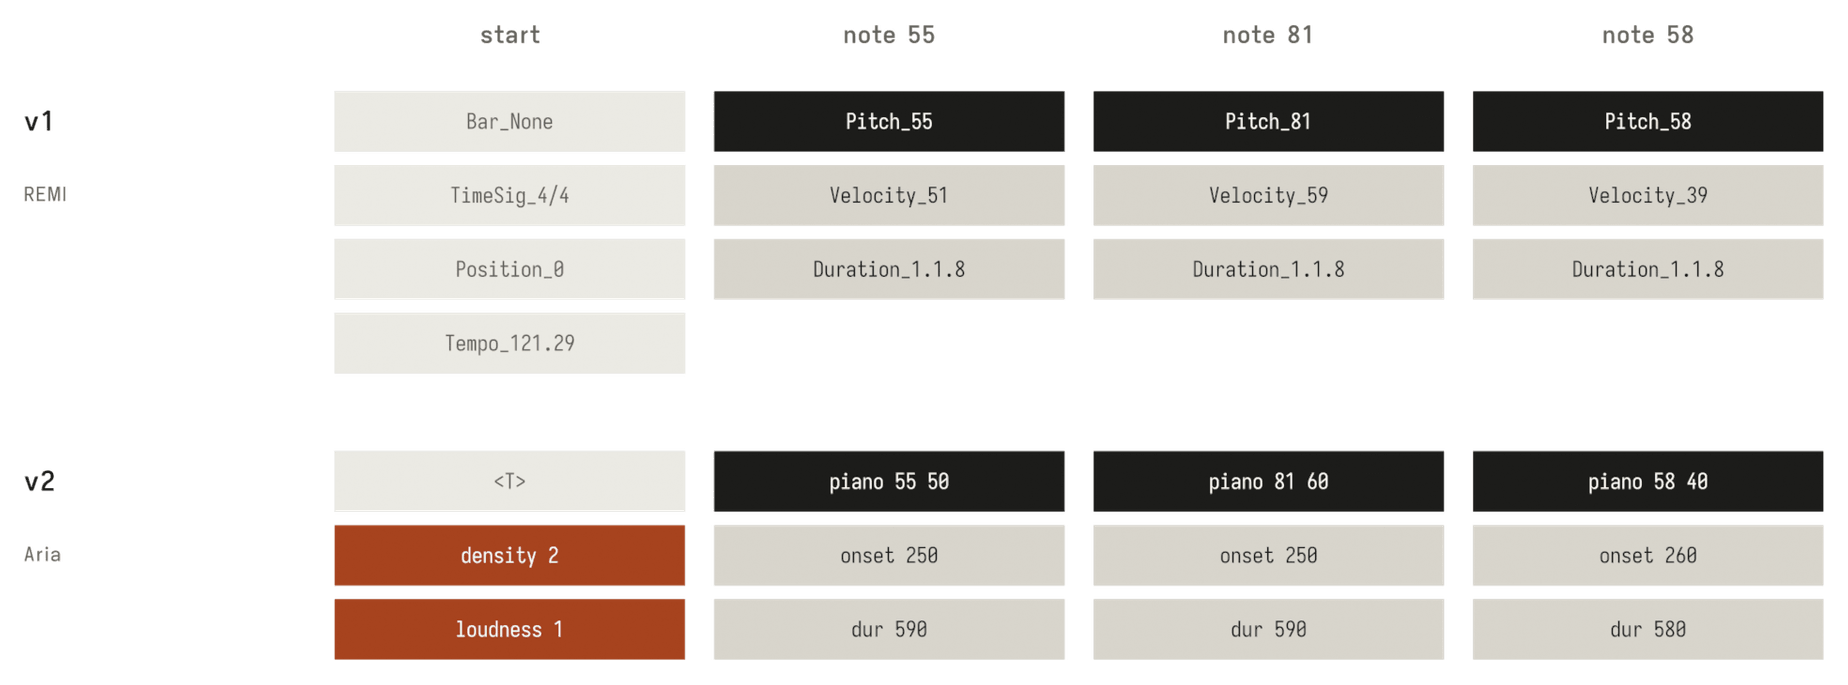
\includegraphics[width=\textwidth]{../figures/tokens-light.png}
\caption{The same three notes in both tokenizations, as the tokenizers write them.}
\end{figure}

\section{Training}

\begin{table}[h]
\centering\small
\begin{tabular}{lp{0.3\textwidth}p{0.48\textwidth}}
\toprule
& v1 & v2 \\
\midrule
Window & 2,048 tokens, stride 1,024 & 1,024 tokens, drawn at random, weighted by file length \\
Batch & 16 windows (32,768 tokens) & 256 windows (262,144 tokens) \\
Optimizer & AdamW, weight decay 0.01 & AdamW, $\beta = (0.9, 0.99)$, weight decay 0.1, clip 1.0 \\
Learning rate & $2\cdot10^{-4}$, 1,000 warmup, cosine & $6\cdot10^{-4}$, 500 warmup, constant, $1-\sqrt{\cdot}$ decay over the last 20\,\% \\
Length & 4 epochs, best epoch kept & 2 passes of 17,509 steps \\
Hardware & RX 9060 XT, bf16 & RX 9060 XT (bf16) and Radeon VII (fp16), gradients summed over gloo \\
Speed & about 20k tokens/s & about 29k tokens/s, 44 h per pass \\
\bottomrule
\end{tabular}
\caption{Training settings of the released weights.}
\end{table}

\textbf{v1.} The original v1 was trained in fp32 on an M1 Max with PyTorch's MPS backend and reached a
validation loss of 1.43 after two epochs (1.53 after four). Its weights were lost. The released weights are a
retraining with the same recipe on a Radeon RX 9060 XT in bf16, using 8 windows times 2 accumulation steps
instead of 2 times 8, which gives the same updates. Like the original, it did best after the second
epoch (1.4131) and got worse after that, so the released weights are from epoch 2.

\textbf{v2, two different GPUs.} Each card runs its own process; after each step the gradients are summed
through host memory (gloo), because RCCL did not work on this pair. The faster card does 20 of the 32
micro-batches per step, the slower 12. Two changes to flash-linear-attention 0.5.2 \cite{fla} were needed on
these AMD cards. Its WKV kernel is tuned for chunks of 64 tokens; chunks of 16 were 4 to 6 times faster here.
And under fp16 the WKV output grew past fp16's maximum of 65,504 (up to 335,000 on about 1\,\% of windows after
6,000 steps). On the fp16 card that made the loss non-finite, and every such step halved the loss scale, until
after about 165 of them the scale reached zero and every step from 9,590 on was lost. The fix runs that kernel in
fp32, lets a rank with a non-finite step sit it out while the other's gradient is rescaled to a full step, and
leaves the loss scale alone after a non-finite forward pass. Training resumed at step 9,823 and logged no
non-finite step after that.

\textbf{v2, second pass.} The first pass ended at a validation loss of 1.7929, still falling by 0.014 per 2,000
steps before its learning-rate decay. The second pass started from the checkpoint before that decay (step 14,007,
weights and optimizer) and ran the same 17,509-step schedule over the same data again.

\section{Results}

\subsection{Validation loss}

\begin{table}[h]
\centering\small
\begin{tabular}{lrrr}
\toprule
Token kind & First pass, before decay & First pass, final & Second pass, final \\
\midrule
note (pitch and velocity) & 2.537 & 2.441 & 2.369 \\
onset & 1.744 & 1.692 & 1.657 \\
duration & 1.325 & 1.288 & 1.263 \\
\texttt{<T>} & 0.446 & 0.374 & 0.362 \\
mean & 1.855 & 1.793 & 1.749 \\
\bottomrule
\end{tabular}
\caption{v2 validation loss (nats per token) on the 256 windows the training log uses. The second-pass column
was evaluated in fp16 with the released code (1.7491; the training log has 1.7493 in bf16).}
\end{table}

Notes carry most of the remaining loss: which pitch comes next is where the music is decided.

v1's validation loss, over the 2,048-token windows of the 63 validation files, was 1.501, 1.413, 1.448 and 1.478
after epochs one to four, while its training loss kept falling to about 1.10.

\subsection{Following the controls}

Tested on the first-pass model, sampling with temperature 1 and top-p 0.95. ``Fresh start'' asks for each
density level from an empty state; the long stream runs 15 minutes and switches the density target every 30
seconds. Guidance runs a second stream with ``none'' controls and uses $\ell_a + \gamma(\ell_a - \ell_b)$.

\begin{table}[h]
\centering\small
\begin{tabular}{rrrrr}
\toprule
$\gamma$ & Fresh start & Minutes 0--4 / 10--14 & Notes/s late, targets 3--5 / 8--12 & Malformed per 1,000 \\
\midrule
0 & 0.93 & 0.92 / 0.88 & 4.2 / 10.3 & 0.00 \\
0.5 & 0.94 & 0.95 / 0.99 & 3.9 / 9.9 & 0.00 \\
1 & 0.99 & 0.99 / 0.97 & 3.9 / 10.0 & 0.01 \\
1.5 & 1.00 & 0.99 / 0.99 & 3.8 / 9.8 & 0.02 \\
2 & 1.00 & 0.99 / 0.99 & 3.8 / 10.1 & 0.03 \\
\bottomrule
\end{tabular}
\caption{Share of 5-s segments in the asked density band.}
\end{table}

Without guidance the music follows every switch within the first 5-s segment after it, and the mean velocity is
33 at the softest setting and 91 at the loudest. The one gap is dense music late in a long stream: 80\,\% of
those segments land in their band without guidance, 98\,\% at $\gamma = 0.5$. The small test models
(Section~\ref{sec:small}) drifted away from ``dense'' after 10 to 30 minutes; this model, trained with hidden
controls, does not. So the default is no guidance, which keeps the cost at one model call per token.

\subsection{Comparison with real playing}

96 recordings from v2's validation split (one file each, no silent five seconds in the first minute) supply the
first 20 seconds; each model continues for 40 seconds without controls or guidance, two samples per piece. A logistic
regression on 22 features of seconds 20 to 60 tries to tell the real continuation from the model's. The features
include key fit, notes outside the key, interval, pitch-class and rhythm variety, leaps, range, loudness spread, note
density, polyphony and how often a short figure repeats. It is scored by five-fold cross-validation grouped by
piece (\texttt{eval/compare.py}). To check that the test separates damage from quality, damaged copies of the
real pieces go through the same test.

\begin{table}[h]
\centering\small
\begin{tabular}{lrrr}
\toprule
& AUC & 95\,\% interval & Model rated more real \\
\midrule
v2, second pass & 0.64 & 0.59--0.69 & 30\,\% \\
v2, first pass & 0.68 & 0.63--0.72 & 24\,\% \\
v2, step 2,000 of the second pass & 0.69 & 0.65--0.73 & 22\,\% \\
\midrule
5\,\% of notes moved by 1--2 semitones & 0.62 & 0.59--0.66 & \\
15\,\% of notes moved & 0.79 & 0.75--0.84 & \\
pitches shuffled & 0.89 & 0.85--0.93 & \\
random timing & 0.99 & 0.99--1.00 & \\
random pitches & 1.00 & 1.00--1.00 & \\
\bottomrule
\end{tabular}
\caption{How well a classifier tells each system from real playing. 0.5 would mean it cannot. Intervals are
bootstrap intervals over pieces (500 resamples). The last column is the share of pieces where the model's
version scores as more real than the real one.}
\end{table}

The second pass is the closest to real playing. Its lead over the first pass is 0.044 AUC with a paired interval
of $-0.002$ to 0.094 over pieces: probably real, not certain with 96 pieces. What still separates it from real
playing is variety, each by about a third of a standard deviation: fewer different intervals, flatter loudness,
less varied note timing and fewer pitch classes. Key fit, notes outside the key, leaps and range do not stand out
any more. The early checkpoint repeats short figures far too often (0.76 standard deviations above real playing).
None of this measures whether the music is pleasant.

\subsection{Speed and memory}

\begin{figure}[h]
\centering
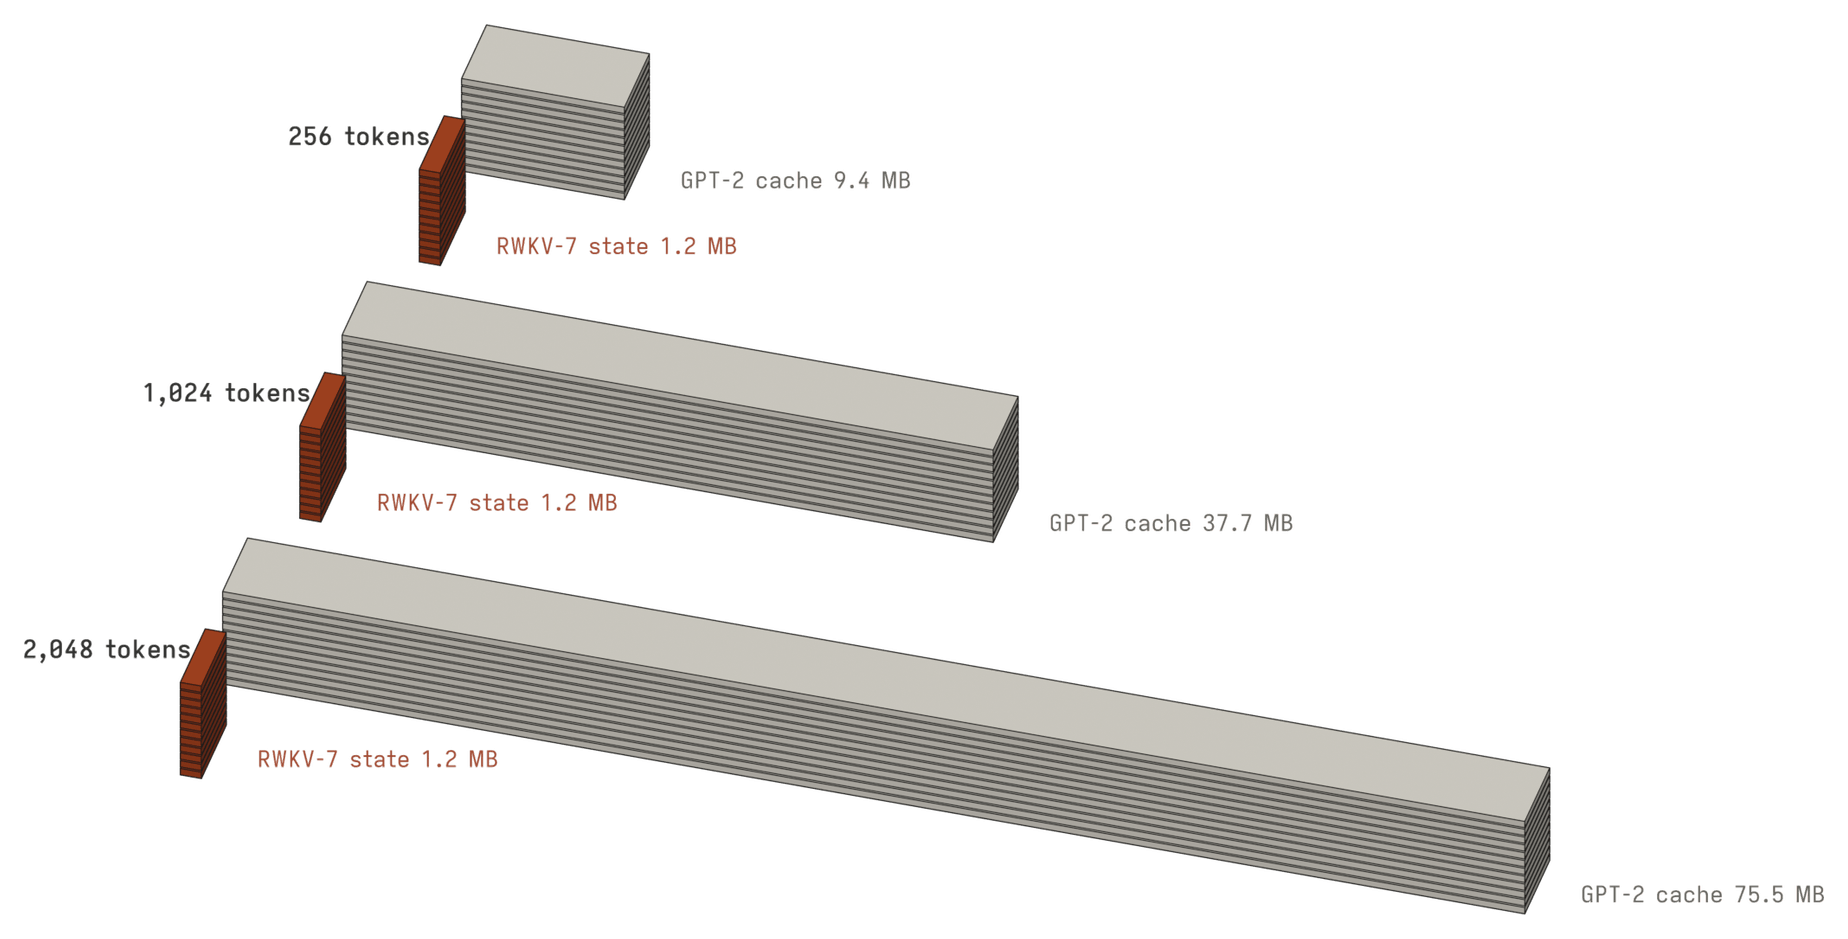
\includegraphics[width=0.8\textwidth]{../figures/memory-light.png}
\caption{Memory per stream in fp16: the GPT-2 key-value cache grows by 36.9 kB per token (12 layers, keys and
values of width 768); the RWKV-7 state is 1.2 MB at any length.}
\end{figure}

Music needs about 30 Aria tokens per second on average and 83 in the busiest 1\,\% of one-second windows, so the
target is about 12 ms per token when generating a second or two ahead. A transformer's growing cache did not
compile for the Neural Engine with Core ML's own stateful API at any size tried, and passing the cache in and out
by hand cost about 13 ms per token (89M parameters, 512-token window). RWKV-7 does the same fixed-shape step for
every token.

\begin{table}[h]
\centering\small
\begin{tabular}{llrrr}
\toprule
Backend & Weights & 1 stream & 2 streams & Top-1 = fp32 \\
\midrule
Neural Engine, Core ML (mains power, 5 Nov) & int8 & 2.86 & 5.73 & 127/128 \\
Neural Engine, Core ML (battery, 26 Oct) & int8 & 4.03 & 7.84 & 502/512 \\
Neural Engine, Core ML (battery, 26 Oct) & fp16 & 5.95 & 11.84 & 506/512 \\
CPU, Core ML (battery, 26 Oct) & int8 & 6.62 & 13.2 & \\
AMX, C + Accelerate (battery, 26 Oct) & fp32 & 10.42 & 12.88 & 512/512 \\
PyTorch CPU, eager & fp32 & 19.1 & & reference \\
\bottomrule
\end{tabular}
\caption{Median time per v2 step in ms on an M1 Pro (2021 MacBook Pro), Low Power Mode off except for the PyTorch
row. The 26 Oct rows used the first-pass weights; the step model is the same.}
\end{table}

\section{Small test runs}
\label{sec:small}

Before the main run, runs of about 28M parameters and 250M tokens chose the architecture and the recipe. They had
no control dropout, so their guidance was contrastive (a second stream with a contrasting control).

\begin{table}[H]
\centering\small
\begin{tabular}{p{0.32\textwidth}p{0.6\textwidth}}
\toprule
Question & Result \\
\midrule
RWKV-7 or GPT with RoPE & validation loss 2.172 against 2.258; at 39M tokens 3.04 against 3.86. A GPT with learned positions was far worse. \\
Density control from a fresh state & asked level hit in 69--97\,\% of segments \\
Loudness control & mean velocity 32 (soft) against 99 (loud) \\
A 35-minute stream without guidance & ``dense'' drifts from 9 to about 5 notes/s after 10--30 minutes in both architectures \\
The same with guidance & $\gamma = 1$ holds ``dense'' at 11 notes/s at minute 15; $\gamma = 2$ overshoots \\
Distillation from Aria (658M) & at most 0.05 nats better at equal tokens and 2.7 times slower: not used \\
Two GPUs against one, 94M & 29.7k against 20.5k tokens/s \\
\bottomrule
\end{tabular}
\caption{Results of the small runs.}
\end{table}

\section{Things that went wrong}

\begin{itemize}
\item The fp16 overflow in the WKV kernel (Section 3) did not crash anything: from step 9,590 the run simply
stopped learning. It was stopped at step 9,823 and resumed with the fix the next morning.
\item Core ML's stateful key-value cache never compiled for the Neural Engine. The RWKV-7 step compiled only once
its per-head norm and sums used rank-3 tensors; with rank-4 tensors Core ML moved it to the CPU without an error.
\item The RX 9060 XT hung twice under an undervolting profile. The run resumed from its 10-minute checkpoint, and
the card has run at stock settings since.
\end{itemize}

\section{Limitations}

\begin{itemize}
\item Neither model plans long-form structure; themes do not come back on their own.
\item v2's controls act every five seconds. Faster changes need a layer outside the model.
\item Aria-MIDI is transcribed from audio and carries transcription errors, and both datasets are mostly classical
piano.
\item The comparison with real playing uses note statistics and 96 pieces; no listener has rated the music.
\item Inference in fp16 on long streams may meet the same overflow as training; the 128-step check does not cover
it.
\item The speed numbers are model steps on one laptop. Running next to a game has not been measured.
\end{itemize}

{\raggedright
\begin{thebibliography}{9}
\bibitem{maestro} C.~Hawthorne et al., ``Enabling Factorized Piano Music Modeling and Generation with the MAESTRO
Dataset,'' ICLR 2019.
\bibitem{ariamidi} L.~Bradshaw and S.~Colton, ``Aria-MIDI: A Dataset of Piano MIDI Files for Symbolic Music
Modeling,'' ICLR 2025.
\bibitem{rwkv7} B.~Peng et al., ``RWKV-7 `Goose' with Expressive Dynamic State Evolution,'' arXiv:2503.14456, 2025.
\bibitem{remi} Y.-S.~Huang and Y.-H.~Yang, ``Pop Music Transformer: Beat-based Modeling and Generation of
Expressive Pop Piano Compositions,'' ACM Multimedia 2020.
\bibitem{miditok} N.~Fradet et al., ``MidiTok: A Python Package for MIDI File Tokenization,'' ISMIR 2021, late-breaking demo.
\bibitem{fla} S.~Yang and Y.~Zhang, flash-linear-attention, \url{https://github.com/fla-org/flash-linear-attention}.
\end{thebibliography}
}

\end{document}
